%%%%%%%%%%%%%%%%%%%%%%%%%%%%%%%%%%%%%%%%%%%%%%%%%%%%%%%
% 
% Machine Learning by Stanford University
% Professor Andrew Ng
% Study Sheet by Reah Miyara <mail@reah.me>
%
%%%%%%%%%%%%%%%%%%%%%%%%%%%%%%%%%%%%%%%%%%%%%%%%%%%%%%%

\documentclass{article}
\usepackage[landscape]{geometry}
\usepackage{url}
\usepackage{multicol}
\usepackage{amsfonts}
\usepackage{tikz}
\usepackage{hyperref}
\usetikzlibrary{decorations.pathmorphing}
\usepackage{amsmath,amssymb}
\usepackage{tikz}
\usetikzlibrary{calc,trees,positioning,arrows,chains,shapes.geometric,%
    decorations.pathreplacing,decorations.pathmorphing,shapes,%
    matrix,shapes.symbols}

\tikzset{
>=stealth',
  punktchain/.style={
    rectangle, 
    rounded corners, 
    % fill=black!10,
    draw=black, thick,
    text width=4em, 
    minimum height=1em, 
    text centered, 
    on chain},
  line/.style={draw, thin, <-},
  element/.style={
    tape,
    top color=white,
    bottom color=blue!50!black!60!,
    minimum width=5em,
    draw=blue!40!black!90, very thick,
    text width=7em, 
    minimum height=2.5em, 
    text centered, 
    on chain},
  every join/.style={->, thick,shorten >=1pt},
  decoration={brace},
  tuborg/.style={decorate},
  tubnode/.style={midway, right=2pt},
}

\usepackage{colortbl}
\usepackage{xcolor}
\usepackage{mathtools}
\usepackage{amsmath,amssymb}
\usepackage{enumitem}
\usepackage[misc]{ifsym}

\title{Machine Learning}
\usepackage[brazilian]{babel}
\usepackage[utf8]{inputenc}

\advance\topmargin-.8in
\advance\textheight3in
\advance\textwidth3in
\advance\oddsidemargin-1.5in
\advance\evensidemargin-1.5in
\newcommand{\sbt}{\,\begin{picture}(-1,1)(-1,-3)\circle*{3}\end{picture}\ }
\parindent0pt
\parskip2pt
\newcommand{\hr}{\centerline{\rule{3.5in}{1pt}}}
%\colorbox[HTML]{e4e4e4}{\makebox[\textwidth-2\fboxsep][l]{texto}
\begin{document}

\begin{center}{\huge{\textbf{Machine Learning by Stanford University}}}\\
	{\large \texttt{Study Sheet by Reah Miyara \href{mailto:mail@reah.me}{\Letter \hspace{3pt}mail@reah.me}}}
\end{center}
\begin{multicols*}{3}
	
	\tikzstyle{mybox} = [draw=black, fill=white, very thick,
	rectangle, rounded corners, inner sep=10pt, inner ysep=10pt]
	\tikzstyle{fancytitle} =[fill=white, text={rgb:yellow,2;green,4;blue,9}, font=\bfseries]
	%------------ Intro to Machine Learning ---------------
	\begin{tikzpicture}
		\node [mybox] (box){%
			\begin{minipage}{0.3\textwidth}
				\textbf{$\sbt$ ML} -- a computer program with increased performance $P$ at some class of tasks $T$ with experience $E$. \\
				\textbf{$\sbt$ Supervised} -- given a [`ground truth'] data set, predict output given the input. Types of prediction:
				\begin{enumerate}
					\itemsep0em 
					\item \textbf{Regression} -- continuous, numerical
					\item \textbf{Classification} -- discrete, categorical  
				\end{enumerate}
				        
				\textbf{$\sbt$ Unsupervised} -- derive structure from data based on relationships among variables (with no prior knowledge as to what the results should look like)
			\end{minipage}
		};
		\node[fancytitle, right=10pt] at (box.north west) {Intro to Machine Learning};
	\end{tikzpicture}
	
	%------------ Linear Regression with One Variable ---------------
	\begin{tikzpicture}
		\node [mybox] (box){%
			\begin{minipage}{0.3\textwidth}
				\textbf{$\sbt$ Learning Goal} -- given a training set, learn a function $h$: X$\rightarrow$Y so $h(x)$ is a good $y$ predictor
				    
				\begin{center}
					\tiny\begin{tikzpicture}
					[node distance=.5cm,
					start chain=going below,]
					\node[punktchain, join] (perfekt) {Training Set};
					\node[punktchain, join, ] (emperi) {Learning Algorithm};
					\node (asym) [punktchain, join ]  {function $h$: X$\rightarrow$Y};
					\begin{scope}[start branch=venstre,
							%We need to redefine the join-style to have the -> turn out right
						every join/.style={->, thick, shorten <=1pt}, ]
						\node[punktchain, on chain=going left, join=by {<-}]
						() {X};
					\end{scope}
					\begin{scope}[start branch=hoejre,]
						\node () [punktchain, on chain=going right, join=by {->}] {prediction Y};
					\end{scope}
					\end{tikzpicture}
				\end{center}
				  
				\textbf{$\sbt$ Hypothesis} -- $h_\theta(x) = \theta_0 + \theta_1x$ \\
				\textbf{$\sbt$ Cost Function} -- takes an average difference of all results of the hypothesis with inputs from the $x$ values and the actual $y$ values. Goal: minimize $\theta_0,\theta_1$\vspace{-10pt}
				\begin{equation}
				J(\theta_0, \theta_1) = \frac{1}{2m}\sum_{i=1}^{m}(h_\theta(x_i)-y_i)^2 
				\vspace{-5pt}\end{equation}
				{\tiny(1) Squared Error function or Mean Squared Error function}\\
				\textbf{$\sbt$ Gradient Descent Algorithm} {\tiny repeat until convergence}
				\vspace{-10pt}\begin{equation}
				\theta_j := \theta_j - \alpha \frac{\partial}{\partial \theta_j} J(\theta_0, \theta_1)
				\end{equation}
			\end{minipage}
		};
		\node[fancytitle, right=10pt] at (box.north west) {Linear Regression with One Variable};
	\end{tikzpicture}
	
	
	\columnbreak
	
%------------ Multivariate Linear Regression ---------------
	\begin{tikzpicture}
		\node [mybox] (box){%
			\begin{minipage}{0.3\textwidth}
				$h_{\theta}(x)$ = 
				$\begin{bmatrix}
					\theta_{0} & \theta_{1} & \dots & \theta_{n}
				\end{bmatrix}$
				$\begin{bmatrix}
					x_{0}\\ 
					x_{1}\\ 
					\vdots\\ 
					x_{n}
				\end{bmatrix}$
				= $\theta^{T}x$
				
				\textbf{$\sbt$ Gradient Descent Algorithm} {\tiny repeat until convergence}
				\vspace{-10pt}\begin{equation}
				\theta_j := \theta_j - \alpha \frac{1}{m}\sum_{i=1}^{m}(h_\theta(x^{(i)}-y^{(i)})\cdot x_j^{(i)} \text{ ; j:= 0\dots n} 
				\end{equation}
				
				\vspace{-5pt}
				\textbf{$\sbt$ Feature Scaling} -- divide the input values by the range (max -- min). Input values in roughly the same range speed up the convergence of gradient descent.\\
				\textbf{$\sbt$ Mean Normalization} -- subtract the mean for an input variable from the values for that input variable.
				\vspace{-8pt}\begin{equation}
				    x_i := \frac{x_i - \mu_i}{s_i}
				\end{equation}
				{\tiny(4) $\mu_i$ is the mean \& $s_i$ is the range, $(max-min)$, of all values for feature $i$ \par}
				
				\textbf{$\sbt$ Learning Rate} -- $\alpha$ too small $\implies$ slow convergence; 
				    $\alpha$ too large $\implies$ may not converge.
			\end{minipage}
			};
		\node[fancytitle, right=10pt] at (box.north west) {Multivariate Linear Regression};
	\end{tikzpicture}
	
%------------ Normal Equation ---------------
	\begin{tikzpicture}
		\node [mybox] (box){%
			\begin{minipage}{0.3\textwidth}
				\textbf{$\sbt$ Normal Equation} -- non-iterative algorithm for minimizing $J(\theta)$; $note:$ O($n^3$)\ to calculate $X^{T}X$\vspace{-8pt}
				\begin{equation}
				    \theta = (X^TX)^{-1}X^Ty
				\end{equation}
				$m$ examples $(x^{(1)},y^{(1)}), \dots, (x^{(m)},y^{(m)})$; $n$ features\\
               			$x^{(i)}$ = 
                			$\begin{bmatrix}
					x^{(i)}_{0}\\
					x^{(i)}_{1}\\
					\vdots\\
					x^{(i)}_{n}
				\end{bmatrix}$
				$\in \mathbb{R}^{n+1}$
				\hspace{3pt}$\vert$\hspace{3pt} 
				X= 
				$\begin{bmatrix}
					(x^{(1)})^T\\
					(x^{(2)})^T\\
					\vdots\\
					(x^{(n)})^T 
				\end{bmatrix}$
				\hspace{3pt}$\vert$\hspace{3pt} 
				y = $\begin{bmatrix}
					y^1\\
					y^2\\
					\vdots\\
					y^m 
				\end{bmatrix}$
				
		{\tiny $x^{(i)}$ = training vector $i$ (containing values from all features); $X$ $\rightarrow$ $m$x(n+1)}\\
		\textbf{$\sbt$ If X$^{T}$X is noninvertible}, common causes include:\par
		\begin{enumerate}
			\itemsep0em 
			\item Redundant features, where two features are very closely related (i.e. they are linearly dependent)
			\item Too many features (e.g. m $\leq$ n). In this case, delete some features or use `regularization'.
		\end{enumerate}
				
			\end{minipage}
		};
		\node[fancytitle, right=10pt] at (box.north west) {Normal Equation};
	\end{tikzpicture}
	

%------------ Classification Logistic Regression ---------------
	\begin{tikzpicture}
		\node [mybox] (box){%
			\begin{minipage}{0.3\textwidth}
				\textbf{$\sbt$ Logistic Regression Model} -- want 0 $\leq$ $h_{\theta}(x) \leq 1$\\
				\vspace{-10pt}\begin{equation}
				    g(z) = \frac{1}{1+e^{-z}}
				\end{equation}
				\textbf{$\sbt$ Sigmoid/Logistic Function}
				\vspace{-10pt}\begin{equation}
				 h_{\theta}(x) = g(\theta^{T}x) = \frac{1}{1+e^{-\theta^{T}(x)}} 
				 \end{equation}
				 \vspace{-20pt}\begin{equation}
				     h_{\theta}(x) = P(y=1 \vert x; \theta) = 1 - P(y=0 \vert x;\theta)
				\end{equation}
		\textbf{$\sbt$ Decision Boundary}\par
		\begin{center}\begin{enumerate}
    			\itemsep0em 
    			\item y = 1 if $\theta^{T}(x) \geq 0$
			\item y = 0 if $\theta^{T}(x) < 0 $
		\end{enumerate}
		\end{center}
		\textbf{$\sbt$ Cost Function}\par
		    \vspace{-20pt}\begin{equation}
			Cost (h_{\theta}(x), y) =
			\begin{cases} 
              -$log$(h_{\theta}(x))& $if $y=1 \\
              -$log$(1-h_{\theta}(x))& $if $y=0 \\
            \end{cases}
            \end{equation}\\\vspace{-30pt}
            \begin{equation}
		Cost(h_\theta(x), y) = -ylog(h_\theta(x))-(1-y)log(1-h_\theta(x))
	    \end{equation}
            \vspace{-15pt}\begin{equation}
			    J(\theta)=\frac{1}{m}\sum_{i = 1}^{m}Cost(h_\theta(x^{(i)}),y^{(i)})
			  \vspace{-8pt}\end{equation}
			{\tiny a vectorized implementation is:}\\
			 \vspace{-20pt}\begin{equation}
			    h=g(X\theta); \hspace{10pt} 
			    J(\theta)=\frac{1}{m} \cdot (-y^{T}log(h)-(1-y)^{T}log(1-h))
			 \end{equation}
			 
			 \vspace{-10pt}\begin{equation}
			    \theta_{j} := \theta_{j} - \frac{\alpha}{m} \sum_{i=1}^{m}(h_{\theta}(x^{(i)})-y^{(i)})\cdot x_{j}^{(i)}
			 \end{equation}
			 {\tiny a vectorized implementation is:}\\
			 \vspace{-10pt}\begin{equation}
			    \theta := \theta - \frac{\alpha}{m} X^{T}(g(X\theta)-\vec{y} )
			    \end{equation}
			\end{minipage}
		};
		\node[fancytitle, right=10pt] at (box.north west) {Classification Logistic Regression};
	\end{tikzpicture}
	
	%------------ Multiclass Classification ---------------
	\begin{tikzpicture}
		\node [mybox] (box){%
			\begin{minipage}{0.3\textwidth}
			\begin{center}
			    y $\in {0, 1, \dots n}$\\
			    h$_\theta^{(0)}(x)$ = P(y=0$\vert$x;$\theta$)\\
			    h$_\theta^{(1)}(x)$ = P(y=1$\vert$x;$\theta$)\\\vspace{-5pt}
			    $\vdots$\\
			    h$_\theta^{(n)}(x)$ = P(y=n$\vert$x;$\theta$)\\
			    prediction = max$_{i}(h_{\theta}^{(i)}(x))$
			\end{center}
			\end{minipage}
		};
		\node[fancytitle, right=10pt] at (box.north west) {Multiclass Classification};
	\end{tikzpicture}
	
	\columnbreak
		%------------ Overfitting ---------------
	\begin{tikzpicture}
		\node [mybox] (box){%
			\begin{minipage}{0.3\textwidth}
			\textbf{$\sbt$ Underfitting} -- hypothesis shows structure not captured by the model; does not fit the data well\\
			\textbf{$\sbt$ Overfitting} -- hypothesis corresponds too closely to data $\therefore$ fail to predict future results reliably\\
			$\sbt$ Addressing the problem of overfitting: \\
			\vspace{-20pt}\begin{enumerate}
			\itemsep0em
			    \item \textbf{Reduce the number of features} -- manually/algorithmically select subset of features.
			    \vspace{-5pt}\item \textbf{Regularization} -- keep all features, but reduce the magnitude of parameters $\theta_j$ by $\lambda$ {\tiny (regularization parameter)}.
			\end{enumerate}
			\vspace{-10pt}\begin{equation}
			        J(\theta) = \frac{1}{2m}\left[ \sum_{i=1}^{m}(h_{\theta}(x^{(i)}) - y^{(i)})^2 + \lambda\sum_{j=1}^{n}\theta^2_j \right]
			\end{equation}
			Gradient Descent {\tiny regularized linear regression does not penalize} $\theta_0$
			\vspace{-10pt}\begin{equation}
		        		\theta_0 := \theta_0-\alpha\frac{1}{m}\sum_{i=1}^{m}(h_{\theta}(x^{(i)}) - y^{(i)})\cdot x^{(i)}_0
			\end{equation}
			\vspace{-10pt}\begin{equation}
		        		\theta_j := \theta_j-\alpha \left[ \left( \frac{1}{m}\sum_{i=1}^{m}(h_{\theta}(x^{(i)}) - y^{(i)})\cdot x^{(i)}_j \right) + \frac{\lambda}{m}\theta_j \right]
			\end{equation}
			\vspace{-15pt}\begin{equation}
		        		\theta_j := \theta_j(1-\alpha \frac{\lambda}{m}) - \alpha \frac{1}{m}\sum_{i=1}^{m}(h_{\theta}(x^{(i)}) - y^{(i)})\cdot x^{(i)}_j 
			\end{equation}

			Normal Equation
			\vspace{-10pt}\begin{equation}
		        		\theta = (X^TX + \lambda \cdot L)^{-1}X^Ty
			\end{equation}
			where L = 
			$\begin{bmatrix}
    				0 & \\
    				& 1 \\
				& & \ddots \\
    				& & & 1
 			\end{bmatrix}$
			\end{minipage}
		};
		\node[fancytitle, right=10pt] at (box.north west) {Under/Over --fitting};
	\end{tikzpicture}

				%------------ Neural Networks ---------------
	\begin{tikzpicture}
		\node [mybox] (box){%
			\begin{minipage}{0.3\textwidth}
			\textbf{$\sbt$ Activation Function}
			\vspace{-10pt}\begin{equation}
				 h_{\theta}(x) = g(\theta^{T}x) = \frac{1}{1+e^{-\theta^{T}(x)}} 
			\vspace{-10pt}\end{equation}
			$a^{(i)}_j$ -- `activation' of unit $i$ in layer $j$\\
			$\Theta^{(j)}$ -- matrix of weights controlling function mapping from layer $j$ to layer $j+1$\\
			\vspace{-10pt}\begin{center}$\begin{bmatrix}
    				x_0\\
    				x_1\\
    				x_2\\
    				x_3\\
 			\end{bmatrix}$
 			$\rightarrow$
 			$\begin{bmatrix}
    				a_1^{(2)}\\
    				a_2^{(2)}\\
    				a_3^{(2)}\\
 			\end{bmatrix}$
 			$\rightarrow$
 			$h_\theta(x)$ \\
 			\end{center}
 			$h_\theta(x)$ = $a_1^{(3)} = g(\Theta^{(2)}_{10}a_0^{(2)} + \Theta^{(2)}_{11}a_1^{(2)} + \Theta^{(2)}_{12}a_2^{(2)} + \Theta^{(2)}_{13}a_3^{(2)})$\\
 			
 			Each layer gets its own matrix of weights, $\Theta^{(j)}$. If network has $s_j$ units in layer $j$ and $s_{j+1}$ units in layer $j+1$, then $\Theta^{(j)}$ will be of dimension $s_{j+1} \times (s_j +1)$.\\

			\textbf{$\sbt$ Forward Propagation: {\tiny vectorized implementation}} --  \\
			    for layer $j=2$ \& node $k$, the variable $z$ will be:\\
			    
			    $z_k^{(2)}$ = $\Theta^{(1)}_{k,0}x_0 + \Theta^{(1)}_{k,1}x_1 + \Theta^{(1)}_{k,n}x_n$\\
			    
			    therefore it follows that: \\
			    
			    $a^{(2)}_1 = g(z_1^{(2)})$, $a^{(2)}_2 = g(z_2^{(2)})$, $a^{(2)}_3 = g(z_2^{(3)})$\\
			    
			    a vectorized representation of $x$ and $z^{(j)}$ is:\\
			    $x = \begin{bmatrix}
    				x_0\\
    				x_1\\
    				\vdots\\
    				x_n\\
 			    \end{bmatrix}$
 			    $z^{(j)} = \begin{bmatrix}
    				z^{j}_1\\
    				z^{j}_2\\
    				\vdots\\
    				z^{j}_n\\
 			    \end{bmatrix}$
 			    \\{\tiny setting $x = a^{(1)}$ we can write it as $z^{(j)} = \Theta^{(j-1)}a^{(j-1)}$ 
 			    $a^{(j)} = g(z^{(j)})$ where g is applied element-wise to our vector $z^{(j)}$
 			    We can then add a bias unit (equal to 1) to layer $j$ after we have computed $a^{(j)}$. This will be $a_0^{(j)}$ and will be equal to 1. To compute our final 			   hypothesis, the last theta matrix $\Theta_{(j)}$ will have only one row which is multiplied by one column $a^{(j)}$ so that our result is a single number. Final 			   result: $h_\Theta(x)=a^{(j+1)}=g(z^{(j+1)})$}
			    \end{minipage}
		};
		\node[fancytitle, right=10pt] at (box.north west) {Neural Networks};
	\end{tikzpicture}

				%------------ Neural Networks ---------------
	\begin{tikzpicture}
		\node [mybox] (box){%
			\begin{minipage}{0.3\textwidth}
				\textbf{$\sbt$ Cost Function \& Backpropagation}
			    	\begin{equation}
			    	\begin{split}
			   	J(\Theta) = -\frac{1}{m}\sum_{i=1}^m \sum_{k=1}^K[y^{(i)}_k log((h_\Theta(x^{(i)}))_k) +\\ 
			    	(1-y^{(i)}_k)log(1-(h_\Theta(x^{(i)}))_k)]+\frac{\lambda}{2m} \sum_{l=1}^{L-1} \sum_{i=1}^{s_l}\sum_{j=1}^{s_{l+1}}(\Theta^{(l)}_{j,i})^2
			    	\end{split}
			    	\end{equation}
				
			    	{\tiny  `Backpropagation' is neural-network term for minimizing our cost function. Given a training set $\{(x^{(1)}, y^{(1)}) \cdots (x^{(m)}, y^{(m)}) \}$:}\\
				{\tiny $\Delta_{i,j}^{(l)} := 0$ for all (l,i,j), (end up with a matrix full of zeros)}\\
				{\tiny for training example t=1 to m:
				\vspace{-7pt}\begin{enumerate}
				\itemsep-.25em
				\item Set $a^{(1)} := x^{(t)}$
				\item Perform forward propagation to compute $a^{(l)}$ for l = 2,3,...,L
				\item Using $y^{(t)}$, compute $\delta^{(L)} = a^{(L)} - y^{(t)}$\\
				L is the total number of layers \& $a^{(L)}$ is the vector of outputs of the activation units for the last later. So our $\delta$ [error values], are the differences of the actual results in the last layer \& the correct outputs in y. For the delta values of the layers before last, use the following equation that steps back from right to left:
				\item $\delta^{(L-1)}, \delta^{(L-2)},..,\delta^{(2)}$ w/ $\delta^{(l)} = ((\Theta^{(l)})^T \delta^{(l+1)}) .\star a^{(l)} .\star (1-a^{(l)})$\\
				delta values of layer l are calculated by multiplying the delta values in the next layer with the theta matrix of layer l. Next, perform element-wise multiplication with function g', the derivative of the activation function g evaluated with the input values given by $z^{(l)}$. $g'(z^{(l)})=a^{(l)} .\star (1-a^{(l)})$ 
				\item $\Delta_{i,j}^{(l)} := \Delta_{i,j}^{(l)} + a_j^{(l)} \delta_i^{(l+1)}$ vectorized as $\Delta^{(l)} := \Delta^{(l)} + \delta^{(l+1)}(a^{(l)})^T$\\
				Hence we update our new $\Delta$ matrix: \\
				$\sbt$ $D^{(l)}_{i,j} := \frac{1}{m}(\delta^{(l)}_{i,j} + \lambda\Theta^{(l)}_{i,j})$ if j $\neq$ 0\\
			        $\sbt$ $D^{(l)}_{i,j} := \frac{1}{m}(\delta^{(l)}_{i,j})$ if j = 0\\
			        The capital-delta matrix D is used as an `accumulator' to add up our values as we go along \& eventually compute our partial derivative $\therefore$ \\
			        $\frac{\partial}{\partial\Theta^{(l)}_{i,j}} J(\Theta)=D^{(l)}_{i,j}$
				\end{enumerate}}
			\end{minipage}
		};
		\node[fancytitle, right=10pt] at (box.north west) {Neural Networks};
	\end{tikzpicture}			
	
					%------------ Evaluating a Learning Algorithm ---------------
	\begin{tikzpicture}
		\node [mybox] (box){%
			\begin{minipage}{0.3\textwidth}
				\textbf{$\sbt$ Debugging a learning algorithm}\\
				{\tiny \vspace{-7pt}\begin{itemize}
				\itemsep-.25em
				\item Getting more training examples -- {\bf fixes high variance}
				\item Trying smaller sets of features -- {\bf fixes high variance}
				\item Adding features -- {\bf fixes high bias}
				\item Adding polynomial features -- {\bf fixes high bias} 
				\item Decreasing $\lambda$ -- {\bf fixes high bias}
				\item Increasing $\lambda$ -- {\bf fixes high variance}
				\end{itemize}}
				{$\sbt$ A hypothesis may have a low error for training examples but still be inaccurate (overfitting). Hence, }\\
				{\tiny \vspace{-7pt}\begin{itemize}
				\itemsep-.25em
				\item Learn $\theta$ and minimize $J_{train}(\Theta)$ using the training set
				\item Compute the test set error $J_{test}(\Theta)$ 
				\end{itemize}}
				\vspace{-5pt}{$\sbt$ Test set error for linear regression: }
				\vspace{-5pt}\begin{equation}
					J_{test}(\Theta) = \frac{1}{2m_{test}}\sum^{m_{test}}_{i=1}(h_{\Theta}(x_{test}^{(i)}) - y^{(i)}_{test})^{2}\vspace{-7pt}
				\end{equation}
				{$\sbt$ Test set error for classification: }
				\begin{center}
				$err(h_{\Theta}(x), y)$ = 1 if $h_{\Theta}(x)$ $\geq$ .5 and y = 0 or $h_{\Theta}(x)$ $<$ .5 and y = 1. Otherwise, $err(h_{\Theta}(x), y)$ = 0. \\
				\end{center}
				$\sbt$ Test Error = $\frac{1}{m_{test}}\sum^{m_{test}}_{i=1}err(h_{\Theta}(x^{(i)}_{test}),y^{(i)}_{test})$
			\end{minipage}
		};
		\node[fancytitle, right=10pt] at (box.north west) {Evaluating a Learning Algorithm};
	\end{tikzpicture}				
	
		
						%------------ Model Selection \& Train/Validation/Test Sets ---------------
	\begin{tikzpicture}
		\node [mybox] (box){%
			\begin{minipage}{0.3\textwidth}
				\textbf{$\sbt$ Model Select and Train/Validation/Test Sets}\\
				{\tiny \begin{enumerate}
				\itemsep-.25em
				\vspace{-10pt}\item Optimize parameters in $\Theta$ using the {\bf training set (60\%)} for each polynomial degree
				\item Find the polynomial degree d with the least error using the {\bf cross validation set (20\%)}
				\item Estimate the generalization error using the {\bf test set (20\%)} with $J_{test}(\Theta^{(d)})$, (d = theta from polynomial with lower error);
				\end{enumerate}}
				\vspace{-5pt}\textbf{$\sbt$ Diagnosing Bias vs. Variance}\\
				{\tiny \begin{itemize}
				\itemsep-.25em
				\vspace{-10pt}\item we need to distinguish whether bias or variance is the problem contributing to bad predictions. 
				\item high bias is underfitting \& high variance is overfitting. Ideally we need to find a golden mean between the two.
				\item training error will tend to decrease as we increase the degree d of the polynomial
				\item cross validation error will tend to decrease as we increase d up to a point, \& then it will increase as d is increased, forming a convex curve.
				\item {\bf High bias (underfitting):} both $J_{train}(\Theta)$ and $J_{CV}(\Theta)$ will be high. Also, $J_{train}(\Theta) \approx J_{CV}(\Theta)$
				\item {\bf High variance (overfitting):} $J_{train}(\Theta)$ will be low and $J_{CV}(\Theta)$ will be much greater than $J_{train}(\Theta)$
				\end{itemize}}
				\vspace{-5pt}\textbf{$\sbt$ Experiencing High Bias}\\
				{\tiny \begin{itemize}
				\itemsep-.25em
				\vspace{-10pt}\item {\bf Low training set size: } $J_{train}(\Theta)$ will be low \& $J_{CV}(\Theta)$ high. 
				\item {\bf Large training set size: } causes both $J_{train}(\Theta)$ \& $J_{CV}(\Theta)$ to be high with $J_{train}(\Theta) \approx J_{CV}(\Theta)$. 
				\item If a learning algorithm is suffering from {\bf high bias, getting more training data will not (by itself) help much}.
				\end{itemize}}
				\vspace{-5pt}\textbf{$\sbt$ Experiencing High Variance}\\
				{\tiny \begin{itemize}
				\itemsep-.25em
				\vspace{-10pt}\item {\bf Low training set size: } $J_{train}(\Theta)$ will be low and $J_{CV}(\Theta)$ high. 
				\item {\bf Large training set size: } $J_{train}(\Theta)$ increases with training set size \& $J_{CV}(\Theta)$ continues to decrease without leveling off. 				Also $J_{train}(\Theta)$ $<$ $J_{CV}(\Theta)$ but the difference between them remains significant. 
				\item If a learning algorithm is suffering from {\bf high variance, getting more training data is likely to help}.
				\end{itemize}}
				\vspace{-15pt}\begin{center}
					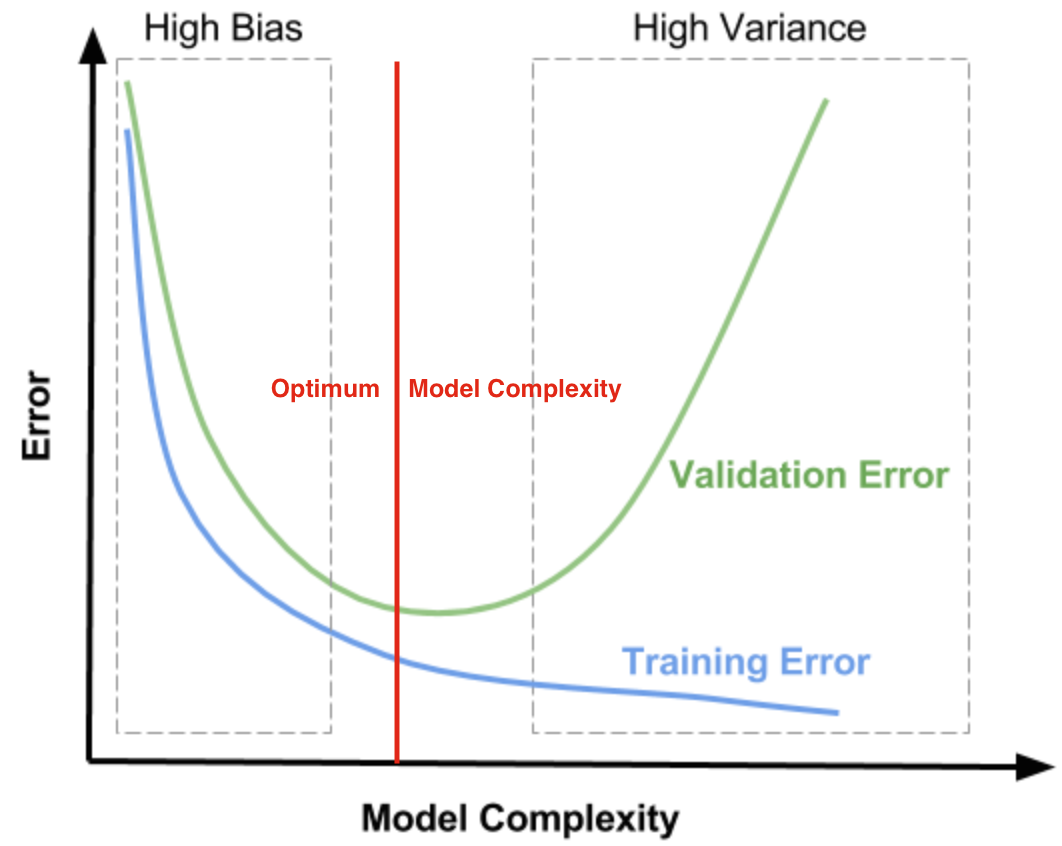
\includegraphics[width=130pt]{cost}
					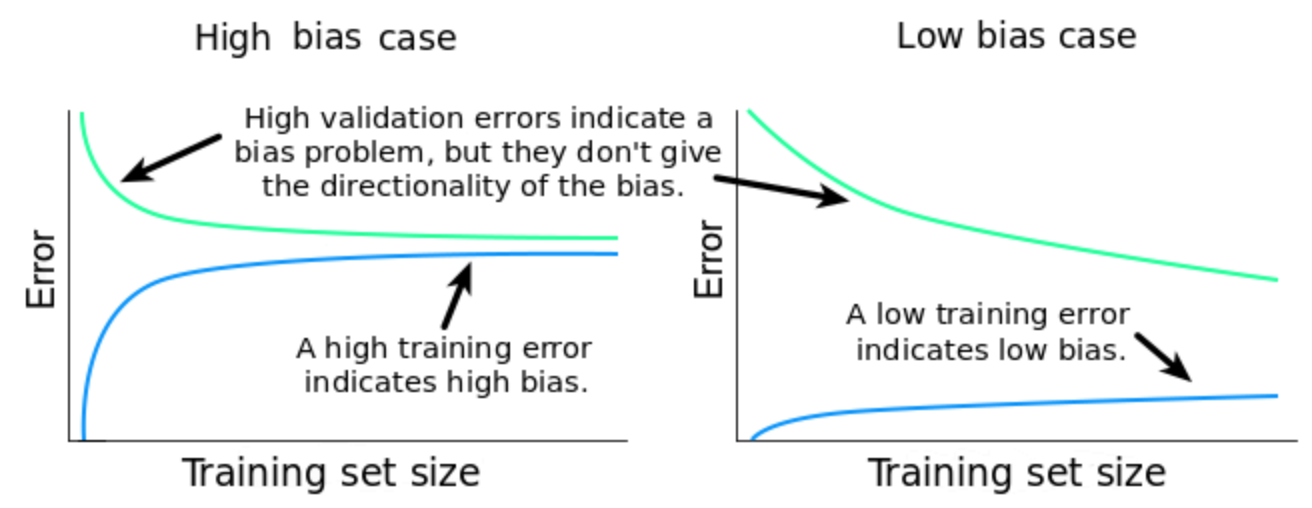
\includegraphics[width=180pt]{bias}
					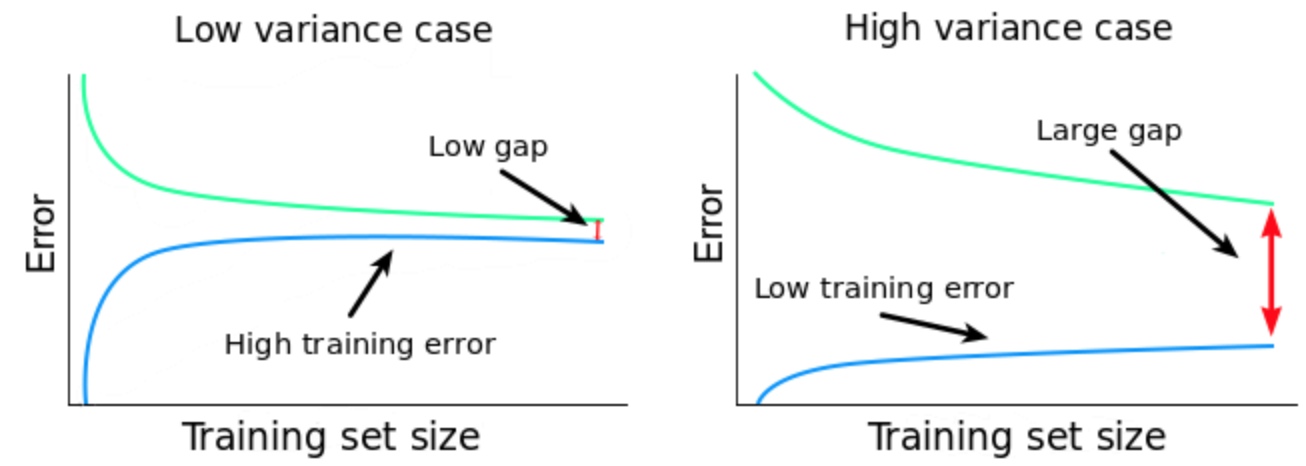
\includegraphics[width=180pt]{variance}
				\end{center}
				\vspace{-5pt}\textbf{$\sbt$ Error Analysis}\\
				{\tiny \begin{enumerate}
				\itemsep-.25em
				\vspace{-10pt}\item Start with a simple algorithm, implement it quickly, and test it early on your cross validation data. 
				\item Plot learning curves to decide if more data, features, etc. will help 
				\item Manually examine the errors on examples in the cross validation set and try to spot a trend where most of the errors were made
				\end{enumerate}}

			\end{minipage}
		};
		\node[fancytitle, right=10pt] at (box.north west) {Evaluating a Learning Algorithm (cont.)};
	\end{tikzpicture}									
	
	
		\end{multicols*}
\end{document}
